%% Document created 12 October 2021 automatically 
%% from /Users/massimosotgia/Desktop/uni_at_DIFI/Lab2/setup.py 

%% Copyright (C) Mattia Sotgia et al. 2022
%% Using class revtex4-2.cls
%                                       
%                                       
%██       █████  ██████         ██████  
%██      ██   ██ ██   ██             ██ 
%██      ███████ ██████          █████  
%██      ██   ██ ██   ██        ██      
%███████ ██   ██ ██████  ██     ███████ 
%                                       
%                                       
\documentclass[
    rmp,
    % preprint,
    % linenumbers,
    % tightlines,
    reprint, 
    superscriptaddress, 
    altaffilletter, 
    amsmath, 
    amssymb, 
    a4paper]{revtex4-2}

\usepackage[top=1.75cm,bottom=2.5cm,left=1.5cm,right=1.5cm]{geometry}

\usepackage[utf8]{inputenc}
\usepackage[T1]{fontenc}

\usepackage[italian]{babel}

%% revtex4-2 bug-fix
\def\andname{e}
%--------------------
\makeatletter
\let\it@comma@def\active@comma
\makeatother

\usepackage{txfonts}
\usepackage{graphicx}% Include figure files
\graphicspath{{../fig/}}

\usepackage{dcolumn}% Align table columns on decimal point
\usepackage{bm}% bold math
\usepackage[colorlinks, urlcolor=., bookmarks]{hyperref}% add hypertext capabilities
\renewcommand\UrlFont{\color{blue}}

\usepackage{physics}
\usepackage{siunitx}

\usepackage{fancyhdr}
\pagestyle{fancy}
\fancyhf{}
\def\twodigits#1{\ifnum#1<10 0\fi\the#1}

%-----------------------------------------------------------------------------------------------

\usepackage{background}
\SetBgColor{gray}
\SetBgAngle{90}
\SetBgScale{2}
\SetBgVshift{0.27\textwidth}

\usepackage[american resistors]{circuitikz}
\usepackage{listings}
\lstset{
  basicstyle=\fontsize{5}{6}\selectfont\ttfamily,
  % backgroundcolor=\color{white},   % choose the background color
  % basicstyle=\footnotesize,        % the size of the fonts that are used for the code
  breakatwhitespace=false,         % sets if automatic breaks should only happen at whitespace
  breaklines=true,                 % sets automatic line breaking
  captionpos=b,                    % sets the caption-position to bottom
  % commentstyle=\color{mygreen},    % comment style
  deletekeywords={...},            % if you want to delete keywords from the given language
  escapeinside={\%*}{*)},          % if you want to add LaTeX within your code
  % extendedchars=true,              % lets you use non-ASCII characters; for 8-bits encodings only, does not work with UTF-8
  % firstnumber=1000,                % start line enumeration with line 1000
  % frame=single,                    % adds a frame around the code
  % keepspaces=true,                 % keeps spaces in text, useful for keeping indentation of code (possibly needs columns=flexible). 
  % keywordstyle=\color{blue},       % keyword style
  % numbers=left,                    % where to put the line-numbers; possible values are (none, left, right)
  % numbersep=5pt,                   % how far the line-numbers are from the code
  numberstyle=\tiny\color{gray}, % the style that is used for the line-numbers
  % rulecolor=\color{black},         % if not set, the frame-color may be changed on line-breaks within not-black text (e.g. comments (green here))
  showspaces=false,                % show spaces everywhere adding particular underscores; it overrides 'showstringspaces'
  showstringspaces=false,          % underline spaces within strings only
  showtabs=false,                  % show tabs within strings adding particular underscores
  stepnumber=2,                    % the step between two line-numbers. If it's 1, each line will be numbered
  % stringstyle=\color{mymauve},     % string literal style
  tabsize=2,                       % sets default tabsize to 2 spaces
}
\usepackage{soul}


%% Define ref types
\newcommand{\reftab}[1]{Tabella {\ref{#1}}}%
\newcommand{\reffig}[1]{Figura {\ref{#1}}}%
\newcommand{\refeqn}[1]{({\ref{#1}})}%
\newcommand{\ChiSqr}{$\chi^2$\space}
\newcommand{\ChiNdf}{$\chi^2/\text{ndf}$}
\newcommand{\cernroot}{\texttt{root}}
\newcommand{\treSigma}{$3\sigma$}
\newcommand{\stdErr}[1]{$\varepsilon_{#1}$}
\newcommand{\mstdErr}[1]{\varepsilon_{#1}}
%% PAPER ONLY custom Macros

\newenvironment{methods}[1]{\section*{#1}
%\fontfamily{phv}
\fontsize{7.5}{9}\selectfont\label{sec:methods}\noindent}{\par\noindent}

%\usepackage{lcsec}


\fancyfoot[C]{
    \the\year\twodigits\month\twodigits\day/1-\thepage
}
\fancyhead[C]{\fontfamily{phv}\fontsize{12}{12}\selectfont RELAZIONE DI LABORATORIO \textbf{
    N. 00 % ! <== CAMBIARE (Nessuna rel. -> 00)
    } (\the\year)
}

\begin{document}

\title{
    Introduzione ai circuiti e studio di filtri del primo ordine
}
\thanks{
    Esperinza n. 1
}

\author{Francesco Polleri}
\email{s5025011@studenti.unige.it}
\altaffiliation{In presenza in laboratorio per la presa dati}
\author{Mattia Sotgia}
\email{s4942225@studenti.unige.it}

\collaboration{Gruppo A1}
\affiliation{Dipartimento di Fisica, Università degli Studi di Genova, I-16146 Genova, Italia}

\date{presa dati
    19 ottobre 2021, analisi dati e relazione in data 
    27 ottobre 2021
}

\begin{abstract}
    Vogliamo costruire e verificare il funzionamento di un filtro passa-basso (\textit{low-pass filter}) o passa-alto (\textit{high-pass filter}) sfruttando i principi fisici che sono dietro al comportamento di un circuito RC posto in tensione alternata.
        
\end{abstract}
\maketitle
\thispagestyle{fancy}
% Rimuovere per consegna
\SetBgContents{
    laboratorio2: e1 (non per la consegna) \today % ! Note di versione
}
\section{Misurazione di $R$}
Con il multimetro da banco impostato per misure di resistenza in corrente continua colleghiamo i capi dei connettori a "banana" al multimetro e alla base di lavoro, quello nero sul GND, quello rosso sul capo +Vcc. 
Mettiamo in serie ai pin corrispondenti al GND e a +Vcc la nostra resistenza ed effettuiamo così la misura del suo valore reale. 

\section{Descrizione apparato sperimentale}
\label{section:introduction}

\begin{figure}[b]
    \begin{circuitikz}
        \ctikzset{bipoles/oscope/width=1.0}
        \draw (4,2)
        node[oscopeshape, fill=gray!20!white](O1){};
        \draw (O1.in 2) to [short, *-] (5,1.2) node[ground]{} node[below left]{GND};
        \draw (0,0)
        node[left]{$V_{in}~1$ V} node[below left=4pt]{(BNC in)} 
        to [short, o-] (0.5,0)
        to [C=$47$ nF] (2.5,0)
        to [R=$1$ k$\Omega$] (2.5,-2) 
        to [short] (0,-2)
        node[ground]{} node[left=4pt]{GND}
        (2.5,0) to [short, -o] node[right]{$V_{out}$} node[below right=4pt]{(BNC out)} (3,0)
        to [short, -] (3,1.2)
        to [short, -*] (O1.in 1);
        \draw [red, dashed] 
        (-2.5,1.8) 
        node[align=left, below right=4pt]{Generatore di\\tensione alternata\\(Oscilloscopio)} 
        rectangle (0.5, -3);
    \end{circuitikz}
    \caption{Circuito utilizzato per il filtro passa-alto progettato nell'esperienza, i valori di R e C sono i valori nominali riportati sul componente.}
    \label{fig:circuit}
\end{figure}

Realizziamo un circuito come quello presente in \reffig{fig:circuit}. Utilizziamo l'oscilloscopio sia come generatore di segnale sinusoidale che come rivelatore. Utilizzando uno sdoppiatore BNC a T possiamo dividere il segnale in uscita, e portare così uno dei due impulsi all'ingresso 1 dello strumento, per poter visualizzare e misurare la tensione in entrata ($v_{in}$) e il suo periodo ($T$). Il secondo cavo BNC lo portiamo ad uno degli ingressi della base di lavoro. In questo modo abbiamo che tutta la base di lavoro viene messa a massa (\hl{\textit{o a terra?}}) e che un pin è posto alla tensione $v_{in}$ alternata.\\
Mettiamo quindi in serie a quest'ultimo il condensatore ($C$) e la resistenza ($R$). Il capo libero della resistenza lo poniamo a massa (\hl{\textit{o a terra?}}).\\
Colleghiamo infine un pin che sia equipotenziale ad un connettore BNC libero con il nodo di collegamento tra C ed R. Colleghiamo il BNC al secondo input presente sull'oscilloscopio per visualizzare il valore di tensione in uscita ($v_{out}$).

Per fornire la tensione di input al sistema con il tasto \verb|Wave Gen| visualizziamo l'interfaccia di generazione del segnale, che impostiamo poi su 1V di ampiezza e lasciamo la frequenza libera di essere variata nel corso della presa dati.

Per effettuare le misure di ampiezza dei segnali che leggiamo con l'oscilloscopio, con il tasto \verb|Meas| accedo all'interfaccia per effettuare misure sul segnale in input. Con i tasti sul basso prima imposto la sorgente del segnale che voglio misurare (1 o 2) che tipo di misura voglio effettuare (ampiezza, periodo, ritardo) e poi imposto con il tasto \verb|Settings| i parametri della misura. 

Impostiamo quattro misure:
\begin{itemize}
    \item Misura della tensione che noi forniano al circuito, che leggiamo con la sorgente 1 dell'oscilloscopio. Impostiamo una misura di ampiezza sulla sorgente 1.
    \item Misura della tensione $v_{out}$, che leggiamo dal secondo ingresso. Impostiamo quindi una misura di ampiezza sulla sorgente 2.
    \item Misura del periodo del segnale, che effettuiamo sul segnale $v_{in}$ poichè osserivamo che ha maggiore stabilità rispetto al segnale in uscita al circuito. Impostiamo una misura di Periodo sulla sorgente 1.
    \item Misura del ritardo del segnale $v_{out}$ rispetto a $v_{in}$. Impostiamo una misura che legga la differenza temporale tra la salita della sorgente 1 e la salita adiacente del segnale 2. 
\end{itemize}

Lo strumento permette di variare l'intervalli orizzontali e verticali in cui misuriamo il segnale per adattarne al meglio la visualizzazione e fornisce i valori di fondo scala relativi per le tensioni e per i tempi, necessari per ricavare l'errore.

\section{Metodi sperimentali}
\begin{table*}
    \begin{ruledtabular}
        \label{table:rawdata}
        \caption{Dati grezzi (sbagliati/pre-correzione)}
        \begin{tabular}{dddddddd}
            \multicolumn{2}{c}{Tensione ingresso (mV)} & \multicolumn{2}{c}{Tensione uscita (mV)} & \multicolumn{2}{c}{Periodo (ms)} & \multicolumn{2}{c}{Ritardo (ms)} \\
            v_{in} & range_{v_{in}} & v_{out} & range_{v_{out}} & T & range_T & dt & range_{dt} \\
            \colrule
            991 & 140 &   4.6 &   2 & 100  & 20    & 20       & 20    \\
            991 & 140 &   7.6 &   2 & 50   & 10    & 11       & 10    \\
            991 & 140 &  15.2 &   3 & 20   & 5     & 4.6      & 5     \\
            991 & 140 &  28   &   4 & 10   & 2     & 2.4      & 2     \\
            993 & 140 &  53   &   8 & 5    & 1     & 1.2      & 1     \\
            991 & 140 & 125   &  18 & 2    & 0.5   & 0.45     & 0.5   \\
            991 & 140 & 243   &  34 & 1    & 0.2   & 0.208    & 0.2   \\
            985 & 140 & 445   &  62 & 0.5  & 0.1   & 0.085    & 0.1   \\
            962 & 140 & 746   & 104 & 0.2  & 0.05  & 0.021    & 0.05  \\
            951 & 140 & 877   & 124 & 0.1  & 0.02  & 0.006    & 0.02  \\
            945 & 140 & 913   & 128 & 0.05 & 0.01  & 0.0016   & 0.01  \\
            946 & 140 & 934   & 140 & 0.02 & 0.005 & 0.00028  & 0.005 \\
            946 & 140 & 940   & 140 & 0.01 & 0.002 & 0.00005  & 0.002 \\
        \end{tabular}
    \end{ruledtabular}
\end{table*}
Dato lo strumento sopra descritto, variando il valore della frequenza del segnale generato, partendo da 10Hz e arrivando a 100kHz rilevando tre valori (1-2-5) per ogni decade, annotiamo i valori di $v_{in}$, $v_{out}$, $T$ e $dt$, con i relativi fondo scala. 

Riportiamo in \reftab{table:rawdata} i valori misurati. 

\section{Calcoli e fit dati}
\begin{table*}
    \begin{ruledtabular}
        \caption{Valori calcolati (sbagliati/pre-correzione)}
        \label{table:cleandata}
        \begin{tabular}{dddddd}
            \multicolumn{2}{c}{Funzione di trasferimento $\left|H[\nu]\right|$ [a. u. ]} & \multicolumn{2}{c}{Fase $\varphi[\nu]$ [rad]} & \multicolumn{2}{c}{Frequenza $\nu$ [Hz]} \\
            \colrule
            0.00464178 & 0.000432655 & 1.25664   & 0.0118382 & 10     & 0.0184752 \\
            0.00766902 & 0.000454563 & 1.3823    & 0.0118859 & 20     & 0.0369504 \\
            0.015338   & 0.000720135 & 1.44513   & 0.0148892 & 50     & 0.11547   \\
            0.0282543  & 0.00105838  & 1.50796   & 0.011938  & 100    & 0.184752  \\
            0.0533736  & 0.00206972  & 1.50796   & 0.011938  & 200    & 0.369504  \\
            0.126135   & 0.00411336  & 1.41372   & 0.0148732 & 500    & 1.1547    \\
            0.245207   & 0.00788168  & 1.3069    & 0.0118568 & 1000   & 1.84752   \\
            0.451777   & 0.0145359   & 1.06814   & 0.0117749 & 2000   & 3.69504   \\
            0.775468   & 0.0252639   & 0.659734  & 0.0145902 & 5000   & 11.547    \\
            0.922187   & 0.0304294   & 0.376991  & 0.0116292 & 10000  & 18.4752   \\
            0.966138   & 0.0318566   & 0.201062  & 0.0116143 & 20000  & 36.9504   \\
            0.987315   & 0.0336198   & 0.0879646 & 0.0145118 & 50000  & 115.47    \\
            0.993658   & 0.0337266   & 0.0314159 & 0.0116085 & 100000 & 184.752   \\
        \end{tabular}
    \end{ruledtabular}
\end{table*}
Vogliamo ottenere il valore della funzione di trasferimento $\left|H[\nu]\right|$, ma poichè si tratta di una funzione complessa preferiamo scriverla in termini del suo modulo e della sua fase. Otteniamo che \[\left|H[\nu]\right|=\frac{v_{in}}{v_{out}}\] e inoltre \[\left|H[\nu]\right|=\frac{1}{\sqrt{1+\frac{1}{R^2 C^2 \omega^2}}}\] che con $\omega_0={1\over{RC}}$ diventa \begin{equation}\left|H[\nu]\right|=\frac{1}{\sqrt{1+\left(\frac{\nu_0}{\nu}\right)^2}} \label{eqn:H}\end{equation} con ${\omega_0\over\omega} = {\nu_0\over\nu}$.

Allo stesso modo per la fase che ottemiamo come \[\varphi[\nu]=2\pi\frac{dt}{T}\] lo possiamo vedere anche come \[\varphi[\nu]=\arctan\left(\frac{1}{RC\omega}\right)\] che diventa \begin{equation} \varphi[\nu]=\arctan\left(\frac{\nu_0}{\nu}\right) \label{eqn:phi}\end{equation} con ${\omega_0\over\omega} = {\nu_0\over\nu}$.

Dal data sheet dello strumeto ricaviamo come calcolare gli errori massimi sui dati misurati che con la regola del \treSigma~ rendiamo statistici. Quindi propaghiamo per ottenere gli errori su $\left|H[\nu]\right|$ e $\varphi[\nu]$.

I valori sono riportati in \reftab{table:cleandata}.

Dalle tabelle ricaviamo un grafico in scala bilogaritmica della funzione di trasferimento rispetto alla frequenza ($\nu$) e un grafico in scala semilogaritmica sulle frequenze di $\varphi[\nu]$ rispetto a $\nu$. Riportiamo in \reffig{fig:plot} il grafico prodotto.

\begin{figure}
    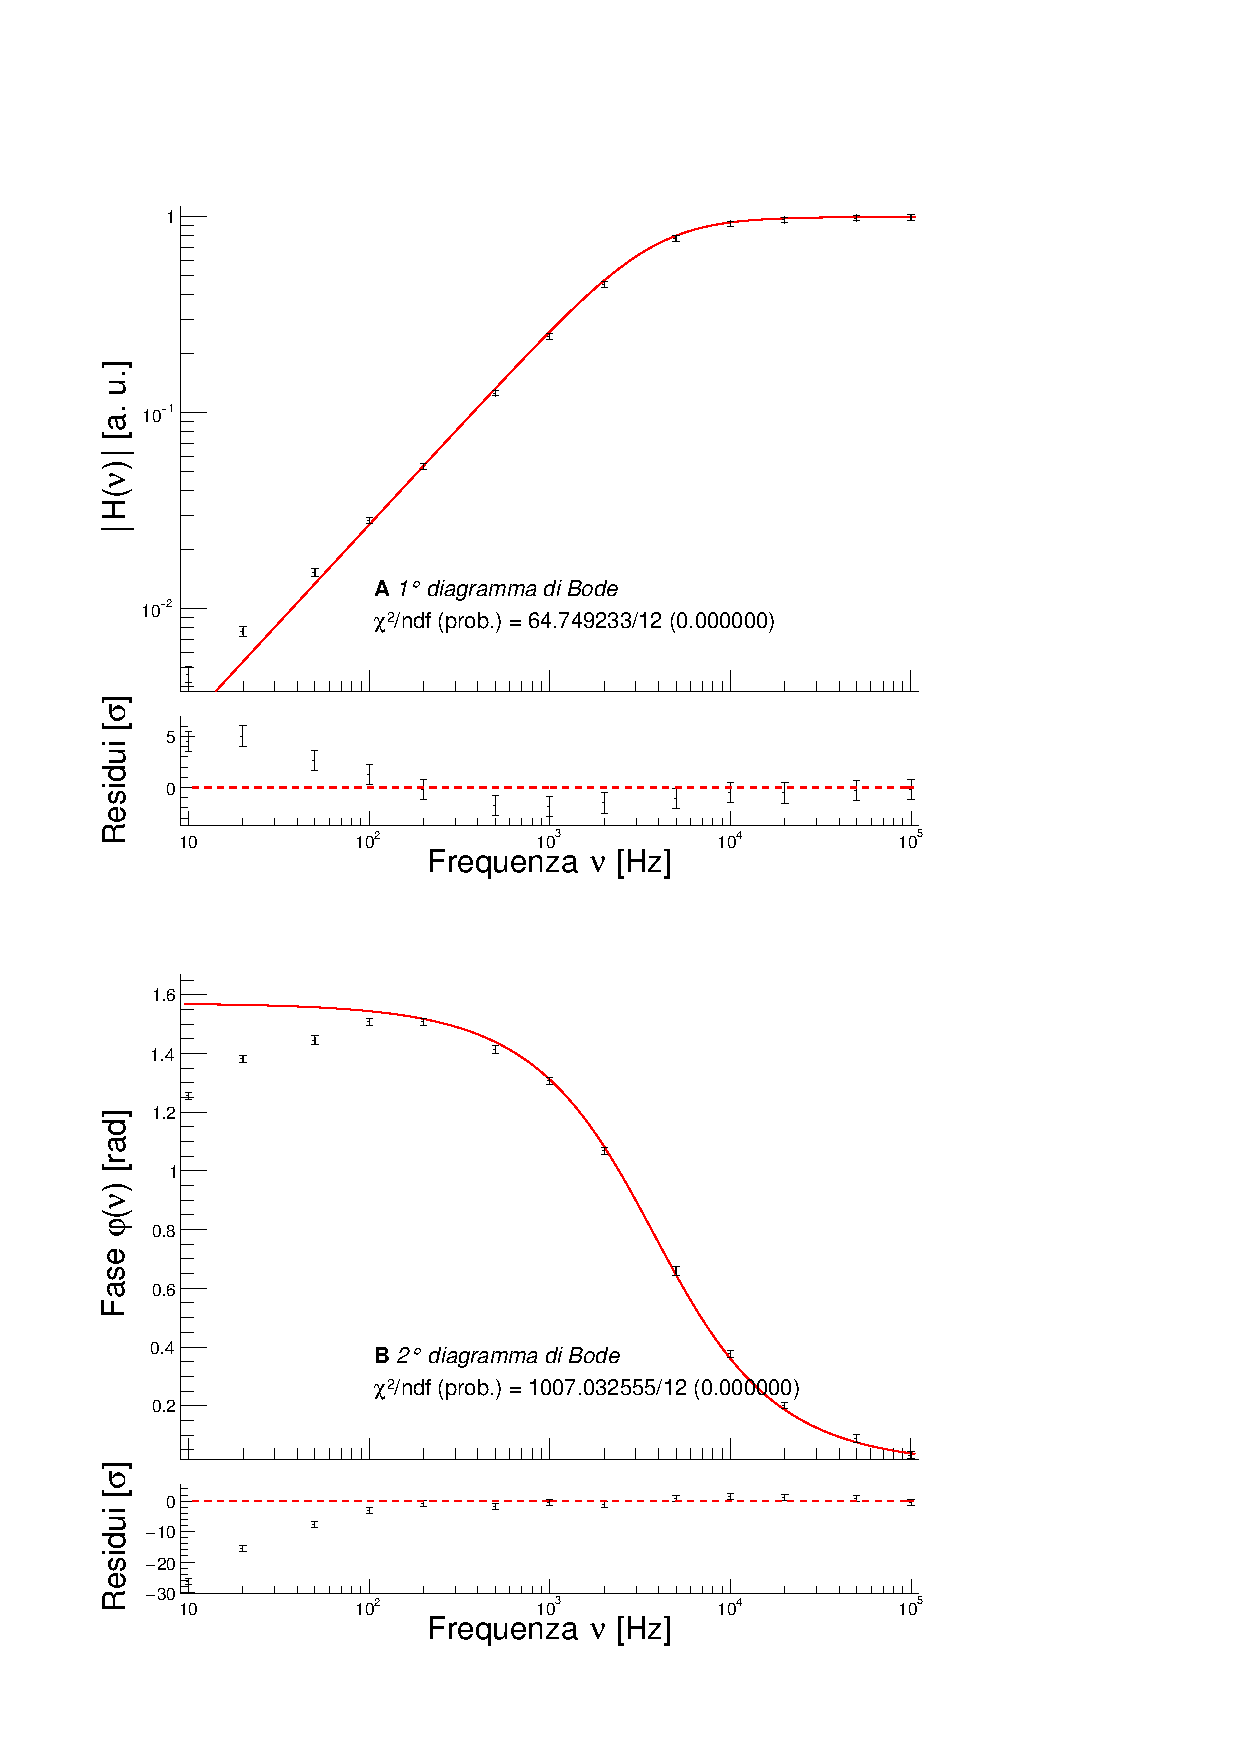
\includegraphics[width=\linewidth]{RC_bode_scorretto.pdf}
    \caption{Diagrammi di Bode, grafico preliminare precedente ad una considerazione sui punti a $\nu<100$Hz.}
    \label{fig:plot}
\end{figure}
\begin{figure}[t]
    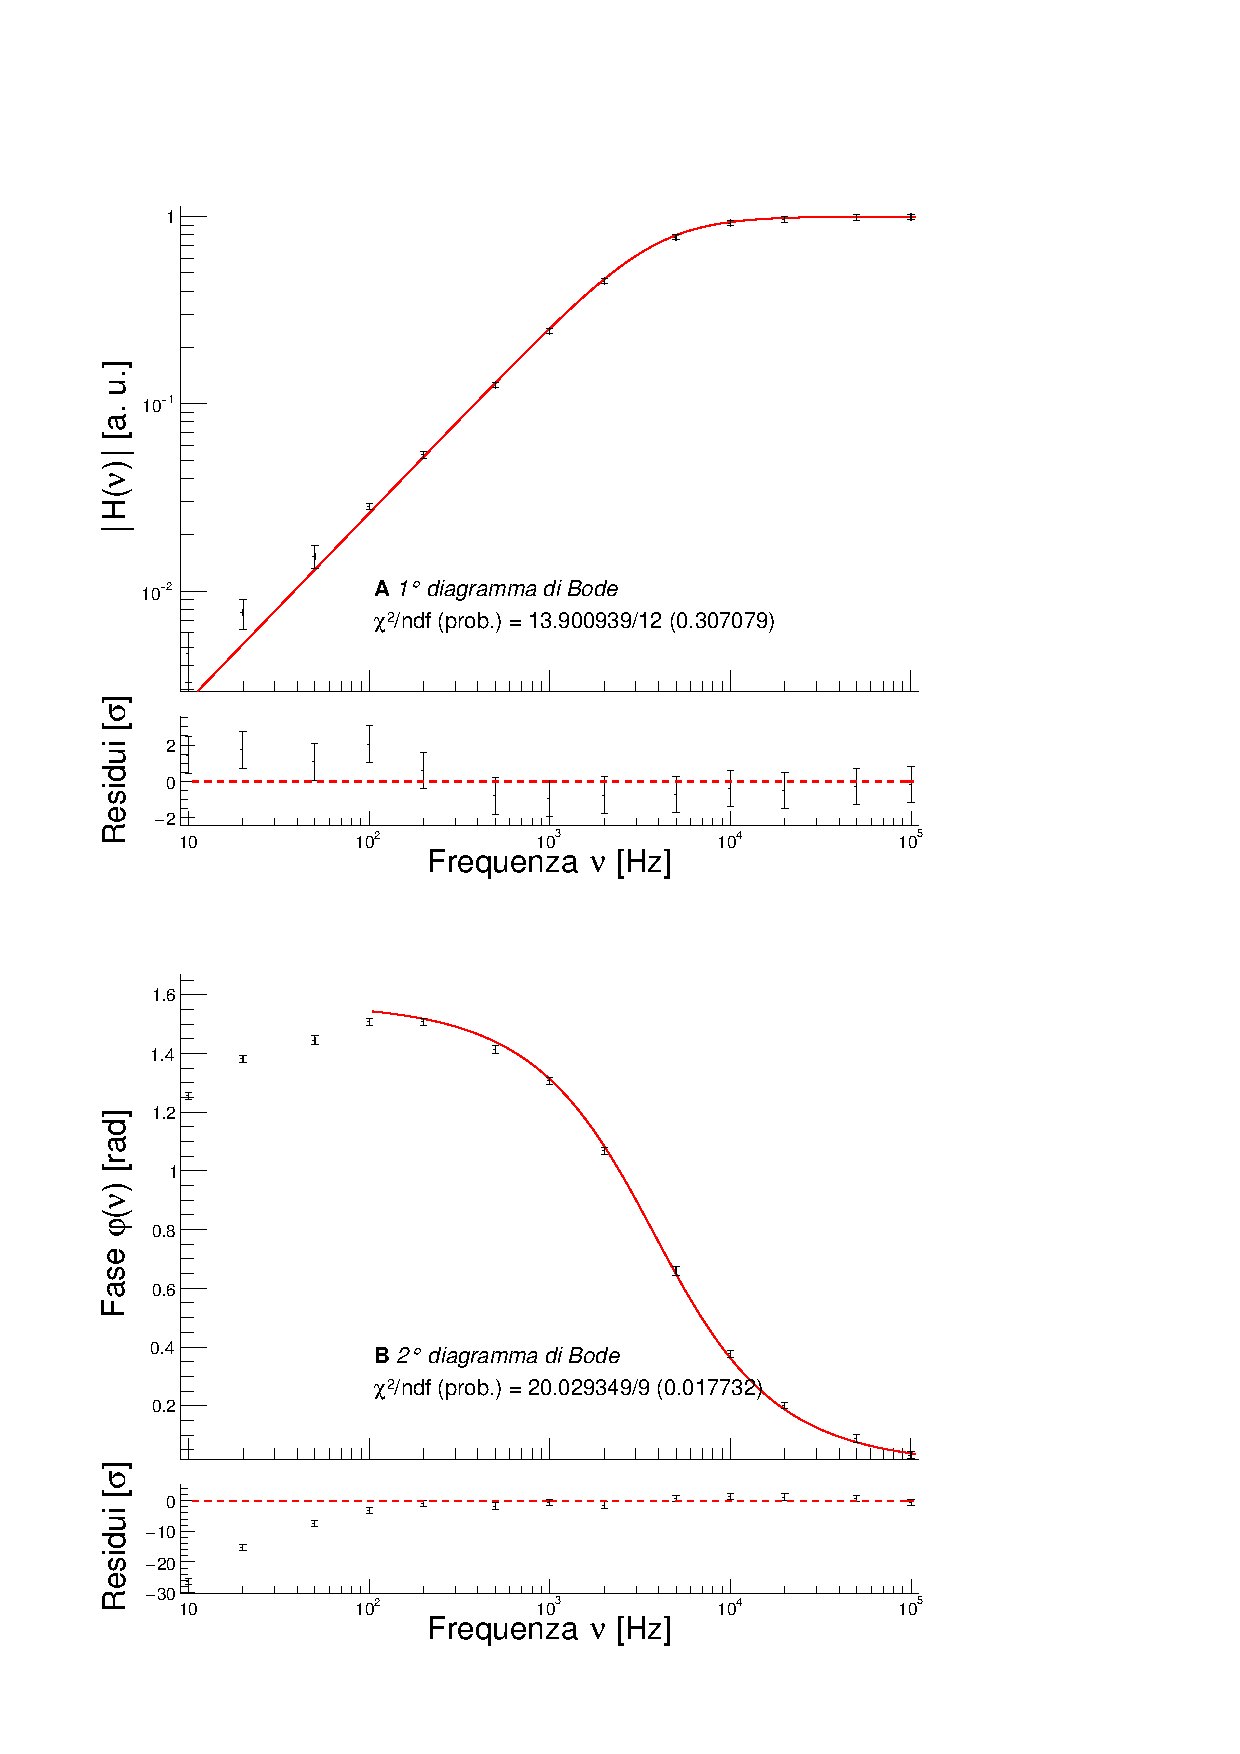
\includegraphics[width=\linewidth]{RC_bode_corretto.pdf}
    \caption{Diagrammi di Bode corretti sui punti a $\nu<100$Hz.}
    \label{fig:plot_correct}
\end{figure}

Eseguiano un fit dei dati sulla base delle funzioni \refeqn{eqn:H} e \refeqn{eqn:phi}, e otteniamo quindi il valore di $\nu_0$ che abbiamo impostato come parametro nella funzione di fit dal I e dal II diagramma di Bode.\\
Analizziamo i valori di \ChiNdf~ e di probabilità del \ChiSqr e osserviamo la compatibilità dei valori trovati. Riportiamo il risultato delle considerazioni e delle operazioni eseguite nell'appendice \ref{appendix:output}.


\section{Considerazioni su rumore a basse frequenze}
\label{sec:correction}
\begin{table*}
    \begin{ruledtabular}
        \caption{Valori calcolati (corretti)}
        \label{table:cleandata_correct}
        \begin{tabular}{dddddd}
            \multicolumn{2}{c}{Funzione di trasferimento $\left|H[\nu]\right|$ [a. u. ]} & \multicolumn{2}{c}{Fase $\varphi[\nu]$ [rad]} & \multicolumn{2}{c}{Frequenza $\nu$ [Hz]} \\
            \colrule
            0.00464178 & 0.00140224 & 1.25664   & 0.0118382 & 10     & 0.0184752 \\
            0.00766902 & 0.00140915 & 1.3823    & 0.0118859 & 20     & 0.0369504 \\
            0.015338   & 0.00212639 & 1.44513   & 0.0148892 & 50     & 0.11547   \\
            0.0282543  & 0.00286993  & 1.50796   & 0.011938  & 100    & 0.184752  \\
            0.0533736  & 0.00206972  & 1.50796   & 0.011938  & 200    & 0.369504  \\
            0.126135   & 0.00411336  & 1.41372   & 0.0148732 & 500    & 1.1547    \\
            0.245207   & 0.00788168  & 1.3069    & 0.0118568 & 1000   & 1.84752   \\
            0.451777   & 0.0145359   & 1.06814   & 0.0117749 & 2000   & 3.69504   \\
            0.775468   & 0.0252639   & 0.659734  & 0.0145902 & 5000   & 11.547    \\
            0.922187   & 0.0304294   & 0.376991  & 0.0116292 & 10000  & 18.4752   \\
            0.966138   & 0.0318566   & 0.201062  & 0.0116143 & 20000  & 36.9504   \\
            0.987315   & 0.0336198   & 0.0879646 & 0.0145118 & 50000  & 115.47    \\
            0.993658   & 0.0337266   & 0.0314159 & 0.0116085 & 100000 & 184.752   \\
        \end{tabular}
    \end{ruledtabular}
\end{table*}
Analizzando il risultato ottenuto dal fit del primo diagramma di Bode, osserviamo che i punti corrispondenti a frequenze minori di 100Hz si discostano in modo evidente dalla curva di fit (lo si vede bene osservando il grafico dei residui). Questo fatto è legato alla presenza di un "rumore" che appunto si manifesta in modo più significativo a basse frequenze perchè la sua ampiezza diventa confrontabile con quella di $v_{out}$. Di conseguenza l'errore da noi impostato, che deriva solamente dal data sheet dello strumento, ci porta a sottostimare molto l'errore su questa misura. Per compensare questa sottostima osserviamo ad occhio, servendoci delle tacche del fondoscala riportate sullo schermo dello strumento, lo spessore della curva del segnale di $v_{out}$. Facendo ciò osserviamo che l'errore vero su questa misura risulta essere circa il 10\% del valore di fondoscala. Impostiamo quindi che tutti i punti a frequenza minore di 100Hz abbiano come errore massimo il 10\% del fondo scala. In tal modo osserviamo che tali punti, attraverso le bande d'errore rientrano nella curva di fit senza modificarla. Riportiamo i valori così calcolati in \reftab{table:cleandata_correct}.

Anche nel secondo diagramma notiamo un comportamento simile dei dati. Tuttavia, poichè la fase è direttamente legata al valore del ritardo, la situazione è più complicata da sistemare. Infatti il ritardo viene misurato dall'oscilloscopio come distanza temporale tra due successive salite del segnale 1 rispetto al segnale 2 però la presenza del rumore può portare lo strumento a confondere la salite del segnale $v_{out}$ con la salita del rumore e non è quindi in grado di dare una lettura corretta di tale intervallo temporale. Inoltre questo errore non è neppure correggibile ad occhio quindi abbiamo preferito impostare come limite per il fit dei dati i punti a frequenza maggiore di 100Hz.


\appendix

\setcounter{table}{0}
\renewcommand{\thetable}{A-\Roman{table}}
\newpage
\section{Output analisi dati prima della correzione}
\label{appendix:output}
\lstinputlisting[]{../misc/results_2021_10_27.log}
\section{Output analisi dati dopo la correzione}
\label{appendix:out_correct}
\lstinputlisting[]{../misc/results_error_correction_2021_10_27.log}

\onecolumngrid
\section{Programma di analisi dati}
\lstinputlisting[language=C]{../analisi_dati/analisi_RC_filter.C}

\end{document}
    
